%!TEX root = ../dokumentation.tex

\chapter{Hazelcast (Key-Value)} \label{ch:hazelcast}
\chapterauthor{Nick Schroeder, Maxime Fritzsch, Michelle Mersch}

Exercitation qui duis voluptate do esse aute. Minim deserunt ex minim sunt cupidatat est fugiat in pariatur ullamco. Enim esse voluptate nulla et sunt sint labore non ut eiusmod et. Deserunt laboris ullamco occaecat esse reprehenderit anim. Deserunt aute laboris tempor est occaecat duis in cupidatat.

\section{Introduction} \label{sec:introductionHazelcast}

\section{Fundamentals} \label{sec:fundamentalsHazelcast}
\subsection{History} \label{subsec:historyHazelcast}
\subsection{Capabilities} \label{subsec:capabilitiesHazelcast}
\subsection{Fields of Application} \label{subsec:fieldsOfApplicationHazelcast}

\section{Implementation} \label{sec:implementationHazelcast}

In the second section of this chapter, a hazelcast cluster will be set up, including a cluster management 
instance. Then, some capabilities are demonstrated using a simple dataset of relational data, highlighting 
the differences between a traditional SQL database.

\subsection{Requirements} \label{subsec:requirementsHazelcast}

To deploy a hazelcast cluster on a local machine, Docker is used, utilising the existing images, 
\enquote{hazelcast/hazelcast} \textcite{Hazelcast.Docker.Hazelcast} and \enquote{hazelcast/management-center} 
\textcite{Hazelcast.Docker.ManagementCenter}. 
Following the official documentation, two member instances are set up alongside a single cluster manager, 
simulating a cluster environment. The cluster manager is then accessible via port 8080, providing status 
information about the cluster members. To fully interact with the cluster, it is necessary to install a 
client. Hazelcast supports a handful of open-source APIs in multiple programming languages. 
\textcite{Hazelcast.Clients} Within the scope of this document, the python client is 
used in the following sections to demonstrate data import and access. The client can get installed with pip 
or any preferred python package manager.

\subsection{Data Import} \label{subsec:dataImportHazelcast}

Once everything is ready, one can import the data into the hazelcast cluster. The following figure displays 
a simple relational data model, which will serve as an example

\begin{figure}[H]
    \caption{Hazelcast Implementation Example} \label{fig:hazelcast.implementation.tables}
    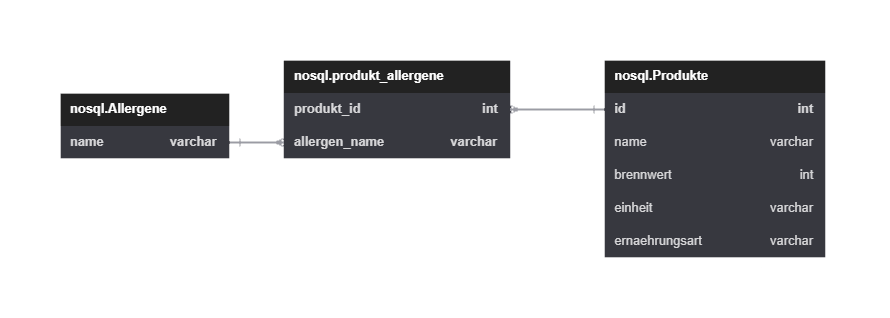
\includegraphics[width=1\textwidth]{images/hazelcast.implementation.tables.png}
    \small\textit{Image generated with \href{https://dbdiagram.io/}{dbdiagram.io}
\end{figure}

\noindent
The table on the left contains only one attribute, the primary key. Depending on the requirements, 
there are two possible data structures to represent this table in a key-value store. The "Set", similar to 
the built-in python data type, is a list of elements. It disallows duplicates, imitating the primary 
key constraint of a relational database. However, as a non-partitioned data structure 
\textcite{Hazelcast.DataStructure.Set}, 
all elements of a single set are kept on one cluster member. Thus, a Set should not be used with large sets. 
The second structure is the "Map". It is a distributed structure and split between single members. 
Additionally, based on the Java Map \textcite{Hazelcast.DataStructure.Map}, its ordinary time 
complexity is quite efficient. \textcite{Hazelcast.Java.Map} 
Therefore, a Map is used to represent the "Allergene" table. However, a synthetic key is required to 
insert and access values. An incremental integer could provide this, as shown in the figure below.


\begin{figure}[H]
    \caption{Hazelcast Implementation Example} \label{fig:hazelcast.allergens.map}
    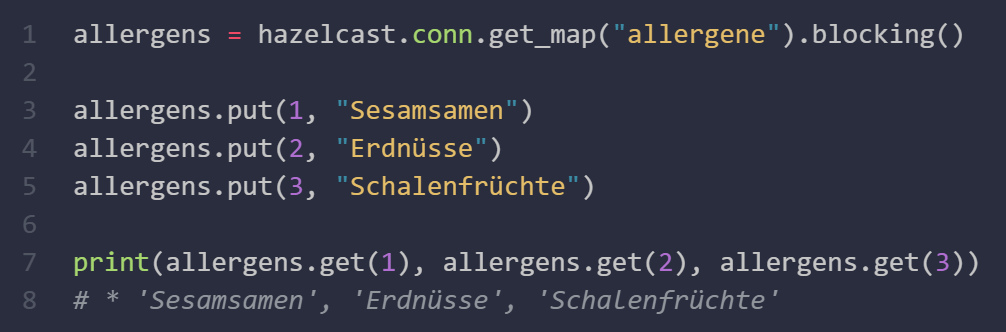
\includegraphics[width=1\textwidth]{images/hazelcast.allergens.map.png}
    \small\textit{Image generated with \href{https://dbdiagram.io/}{dbdiagram.io}
\end{figure}

Not only can Map store primitive values such as integers or strings, but also more complex ones, for 
example, JSON Objects. The python client can readily encode JSON Objects and store them on the cluster, 
which will be used for the "Products" table.

\begin{figure}[H]
    \caption{Hazelcast Implementation Example} \label{fig:hazelcast.products.map}
    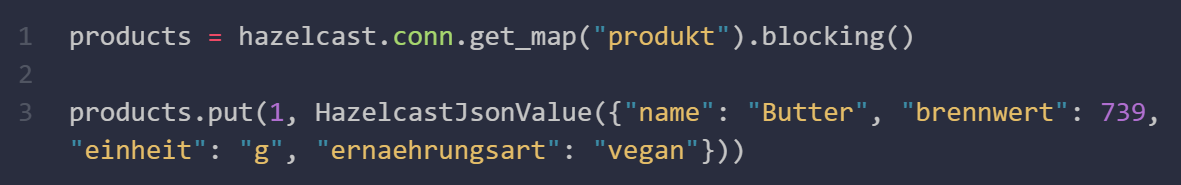
\includegraphics[width=1\textwidth]{images/hazelcast.products.map.png}
    \small\textit{Image generated with \href{https://dbdiagram.io/}{dbdiagram.io}
\end{figure}

\textcite{Hazelcast.PythonClient.HazelcastJsonValue}
Nevertheless, to insert new values, an application has to keep track of the current integer key and check 
for duplicates since a map does not enforce unique values. Additionally, as Maps are meant to be flexible, 
they do not enforce type constraints. Therefore, data validation should be handled by an application before 
manipulating data on the cluster.
The last table, "produkt_allergene", represents a many-to-many relation and therefore holds entries with the 
same "produkt_id" but different "allergen_name", as one product may contain multiple allergens.
Using a Map and manually encoding a list of allergens similar to that shown in \autoref{fig:hazelcast.allergens.map} 
would be possible. Since all allergens are known at the time of creation, the 
list is not updated frequently. However, if the list is regularly updated or contains many elements, it 
would be required to load all entries on the application side, manipulate it and overwrite the old version 
on the hazelcast cluster. 
Thus, hazelcast supports "MultiMaps", another distributed key-value data structure that is able to hold 
multiple values per key, preventing duplicates for one key. \textcite{Hazelcast.DataStructure.MultiMap} 
An example of inserting elements into a MultiMap is shown below.

\begin{figure}[H]
    \caption{Hazelcast Implementation Example} \label{fig:hazelcast.product_allergens.1.multimap}
    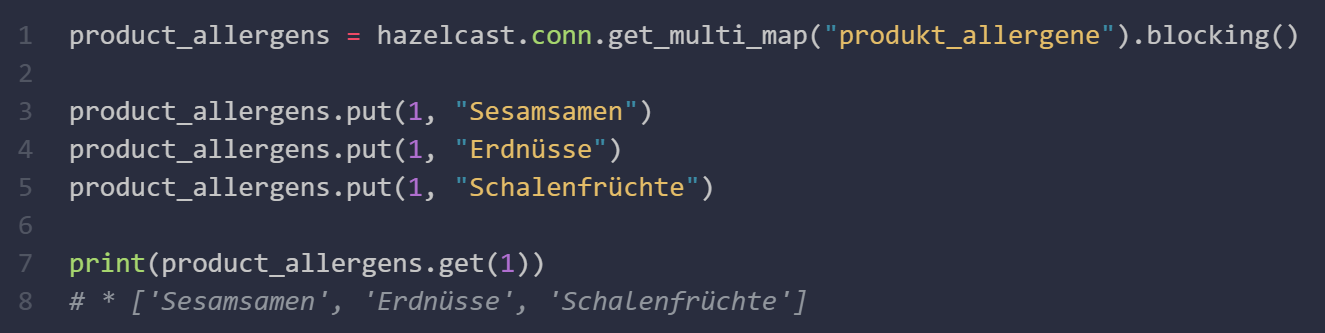
\includegraphics[width=1\textwidth]{images/hazelcast.product_allergens.multimap.1.png}
    \small\textit{Image generated with \href{https://dbdiagram.io/}{dbdiagram.io}
\end{figure}

\subsection{Data Access} \label{subsec:dataAccessHazelcast}

When it comes to accessing data, problems may occur if the key of a particular entry is unknown or one wants 
to query an entire map for multiple key-value pairs that fulfil certain conditions. For such use cases, 
hazelcast offers "Predicates", methods similar to SQL to query a cluster. \textcite{Hazelcast.Predicates} 
A small sample of their capabilities is shown below. 

\begin{figure}[H]
    \caption{Hazelcast Implementation Example} \label{fig:hazelcast.predicates}
    \includegraphics[width=1\textwidth]{images/hazelcast.product_allergens.multimap.png}
    \small\textit{Image generated with \href{https://dbdiagram.io/}{dbdiagram.io}
\end{figure}

Nonetheless, referring back to the "produkt_allergene" table, one might not only want to know all 
allergens of one particular product but also all products which contain one particular allergen. 
Depending on the use case, it may therefore be useful to create copies of maps and rearrange them 
to simplify access to data from multiple perspectives. 

\begin{figure}[H]
    \caption{Hazelcast Implementation Example} \label{fig:hazelcast.product_allergens.2.multimap}
    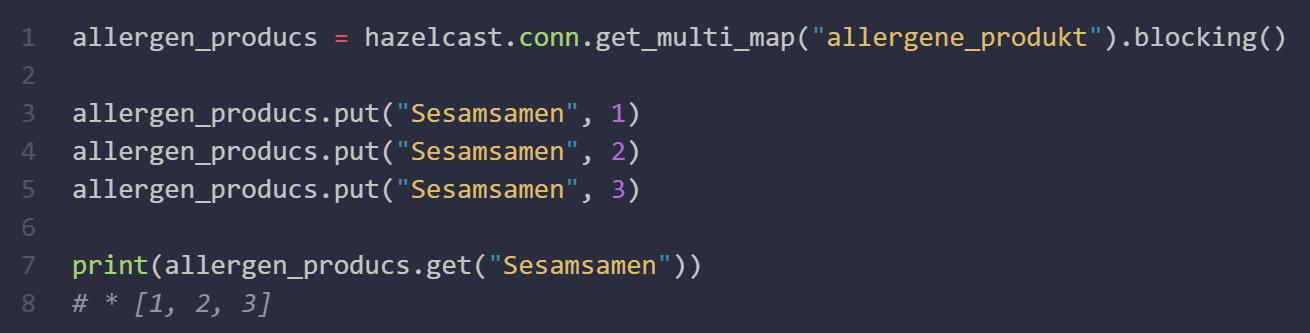
\includegraphics[width=1\textwidth]{images/hazelcast.product_allergens.multimap.2.png}
    \small\textit{Image generated with \href{https://dbdiagram.io/}{dbdiagram.io}
\end{figure}




\section{Reflection} \label{sec:reflectionHazelcast}
\subsection{Advantages \& Disadvantages} \label{subsec:advantagesDisadvantagesHazelcast}
\subsection{CAP Theorem} \label{subsec:capTheoremHazelcast}
\subsection{Conclusion} \label{subsec:conclusionHazelcast}

